% REV00 Tue 04 May 2021 13:55:16 WIB
% START Tue 04 May 2021 13:55:16 WIB

\chapter{XXX}

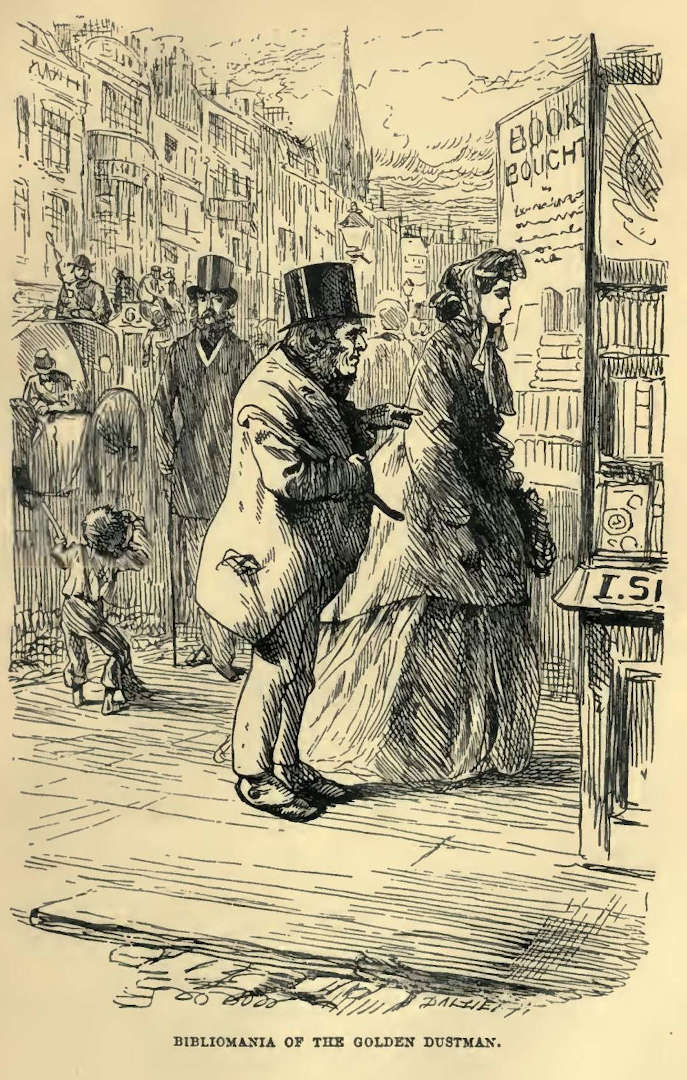
\includegraphics[scale=2.3]{03-05-01}

Chapter 5

THE GOLDEN DUSTMAN FALLS INTO BAD COMPANY


Were Bella Wilfer’s bright and ready little wits at fault, or was the
Golden Dustman passing through the furnace of proof and coming out
dross? Ill news travels fast. We shall know full soon.

On that very night of her return from the Happy Return, something
chanced which Bella closely followed with her eyes and ears. There was
an apartment at the side of the Boffin mansion, known as Mr Boffin’s
room. Far less grand than the rest of the house, it was far more
comfortable, being pervaded by a certain air of homely snugness, which
upholstering despotism had banished to that spot when it inexorably set
its face against Mr Boffin’s appeals for mercy in behalf of any other
chamber. Thus, although a room of modest situation--for its windows gave
on Silas Wegg’s old corner--and of no pretensions to velvet, satin, or
gilding, it had got itself established in a domestic position analogous
to that of an easy dressing-gown or pair of slippers; and whenever the
family wanted to enjoy a particularly pleasant fireside evening, they
enjoyed it, as an institution that must be, in Mr Boffin’s room.

Mr and Mrs Boffin were reported sitting in this room, when Bella got
back. Entering it, she found the Secretary there too; in official
attendance it would appear, for he was standing with some papers in his
hand by a table with shaded candles on it, at which Mr Boffin was seated
thrown back in his easy chair.

‘You are busy, sir,’ said Bella, hesitating at the door.

‘Not at all, my dear, not at all. You’re one of ourselves. We never
make company of you. Come in, come in. Here’s the old lady in her usual
place.’

Mrs Boffin adding her nod and smile of welcome to Mr Boffin’s words,
Bella took her book to a chair in the fireside corner, by Mrs Boffin’s
work-table. Mr Boffin’s station was on the opposite side.

‘Now, Rokesmith,’ said the Golden Dustman, so sharply rapping the table
to bespeak his attention as Bella turned the leaves of her book, that
she started; ‘where were we?’

‘You were saying, sir,’ returned the Secretary, with an air of some
reluctance and a glance towards those others who were present, ‘that you
considered the time had come for fixing my salary.’

‘Don’t be above calling it wages, man,’ said Mr Boffin, testily. ‘What
the deuce! I never talked of any salary when I was in service.’

‘My wages,’ said the Secretary, correcting himself.

‘Rokesmith, you are not proud, I hope?’ observed Mr Boffin, eyeing him
askance.

‘I hope not, sir.’

‘Because I never was, when I was poor,’ said Mr Boffin. ‘Poverty and
pride don’t go at all well together. Mind that. How can they go well
together? Why it stands to reason. A man, being poor, has nothing to be
proud of. It’s nonsense.’

With a slight inclination of his head, and a look of some surprise,
the Secretary seemed to assent by forming the syllables of the word
‘nonsense’ on his lips.

‘Now, concerning these same wages,’ said Mr Boffin. ‘Sit down.’

The Secretary sat down.

‘Why didn’t you sit down before?’ asked Mr Boffin, distrustfully. ‘I
hope that wasn’t pride? But about these wages. Now, I’ve gone into the
matter, and I say two hundred a year. What do you think of it? Do you
think it’s enough?’

‘Thank you. It is a fair proposal.’

‘I don’t say, you know,’ Mr Boffin stipulated, ‘but what it may be more
than enough. And I’ll tell you why, Rokesmith. A man of property, like
me, is bound to consider the market-price. At first I didn’t enter into
that as much as I might have done; but I’ve got acquainted with other
men of property since, and I’ve got acquainted with the duties of
property. I mustn’t go putting the market-price up, because money may
happen not to be an object with me. A sheep is worth so much in the
market, and I ought to give it and no more. A secretary is worth so much
in the market, and I ought to give it and no more. However, I don’t mind
stretching a point with you.’

‘Mr Boffin, you are very good,’ replied the Secretary, with an effort.

‘Then we put the figure,’ said Mr Boffin, ‘at two hundred a year.
Then the figure’s disposed of. Now, there must be no misunderstanding
regarding what I buy for two hundred a year. If I pay for a sheep, I buy
it out and out. Similarly, if I pay for a secretary, I buy HIM out and
out.’

‘In other words, you purchase my whole time?’

‘Certainly I do. Look here,’ said Mr Boffin, ‘it ain’t that I want to
occupy your whole time; you can take up a book for a minute or two when
you’ve nothing better to do, though I think you’ll a’most always find
something useful to do. But I want to keep you in attendance. It’s
convenient to have you at all times ready on the premises. Therefore,
betwixt your breakfast and your supper,--on the premises I expect to
find you.’

The Secretary bowed.

‘In bygone days, when I was in service myself,’ said Mr Boffin, ‘I
couldn’t go cutting about at my will and pleasure, and you won’t expect
to go cutting about at your will and pleasure. You’ve rather got into
a habit of that, lately; but perhaps it was for want of a right
specification betwixt us. Now, let there be a right specification
betwixt us, and let it be this. If you want leave, ask for it.’

Again the Secretary bowed. His manner was uneasy and astonished, and
showed a sense of humiliation.

‘I’ll have a bell,’ said Mr Boffin, ‘hung from this room to yours,
and when I want you, I’ll touch it. I don’t call to mind that I have
anything more to say at the present moment.’

The Secretary rose, gathered up his papers, and withdrew. Bella’s eyes
followed him to the door, lighted on Mr Boffin complacently thrown back
in his easy chair, and drooped over her book.

‘I have let that chap, that young man of mine,’ said Mr Boffin, taking a
trot up and down the room, ‘get above his work. It won’t do. I must have
him down a peg. A man of property owes a duty to other men of property,
and must look sharp after his inferiors.’

Bella felt that Mrs Boffin was not comfortable, and that the eyes of
that good creature sought to discover from her face what attention she
had given to this discourse, and what impression it had made upon her.
For which reason Bella’s eyes drooped more engrossedly over her book,
and she turned the page with an air of profound absorption in it.

‘Noddy,’ said Mrs Boffin, after thoughtfully pausing in her work.

‘My dear,’ returned the Golden Dustman, stopping short in his trot.

‘Excuse my putting it to you, Noddy, but now really! Haven’t you been
a little strict with Mr Rokesmith to-night? Haven’t you been a
little--just a little little--not quite like your old self?’

‘Why, old woman, I hope so,’ returned Mr Boffin, cheerfully, if not
boastfully.

‘Hope so, deary?’

‘Our old selves wouldn’t do here, old lady. Haven’t you found that out
yet? Our old selves would be fit for nothing here but to be robbed and
imposed upon. Our old selves weren’t people of fortune; our new selves
are; it’s a great difference.’

‘Ah!’ said Mrs Boffin, pausing in her work again, softly to draw a long
breath and to look at the fire. ‘A great difference.’

‘And we must be up to the difference,’ pursued her husband; ‘we must be
equal to the change; that’s what we must be. We’ve got to hold our own
now, against everybody (for everybody’s hand is stretched out to be
dipped into our pockets), and we have got to recollect that money makes
money, as well as makes everything else.’

‘Mentioning recollecting,’ said Mrs Boffin, with her work abandoned,
her eyes upon the fire, and her chin upon her hand, ‘do you recollect,
Noddy, how you said to Mr Rokesmith when he first came to see us at the
Bower, and you engaged him--how you said to him that if it had pleased
Heaven to send John Harmon to his fortune safe, we could have been
content with the one Mound which was our legacy, and should never have
wanted the rest?’

‘Ay, I remember, old lady. But we hadn’t tried what it was to have the
rest then. Our new shoes had come home, but we hadn’t put ‘em on. We’re
wearing ‘em now, we’re wearing ‘em, and must step out accordingly.’

Mrs Boffin took up her work again, and plied her needle in silence.

‘As to Rokesmith, that young man of mine,’ said Mr Boffin, dropping
his voice and glancing towards the door with an apprehension of being
overheard by some eavesdropper there, ‘it’s the same with him as with
the footmen. I have found out that you must either scrunch them, or let
them scrunch you. If you ain’t imperious with ‘em, they won’t believe
in your being any better than themselves, if as good, after the stories
(lies mostly) that they have heard of your beginnings. There’s nothing
betwixt stiffening yourself up, and throwing yourself away; take my word
for that, old lady.’

Bella ventured for a moment to look stealthily towards him under her
eyelashes, and she saw a dark cloud of suspicion, covetousness, and
conceit, overshadowing the once open face.

‘Hows’ever,’ said he, ‘this isn’t entertaining to Miss Bella. Is it,
Bella?’

A deceiving Bella she was, to look at him with that pensively abstracted
air, as if her mind were full of her book, and she had not heard a
single word!

‘Hah! Better employed than to attend to it,’ said Mr Boffin. ‘That’s
right, that’s right. Especially as you have no call to be told how to
value yourself, my dear.’

Colouring a little under this compliment, Bella returned, ‘I hope sir,
you don’t think me vain?’

‘Not a bit, my dear,’ said Mr Boffin. ‘But I think it’s very creditable
in you, at your age, to be so well up with the pace of the world, and to
know what to go in for. You are right. Go in for money, my love. Money’s
the article. You’ll make money of your good looks, and of the money Mrs
Boffin and me will have the pleasure of settling upon you, and you’ll
live and die rich. That’s the state to live and die in!’ said Mr Boffin,
in an unctuous manner. ‘R--r--rich!’

There was an expression of distress in Mrs Boffin’s face, as, after
watching her husband’s, she turned to their adopted girl, and said:

‘Don’t mind him, Bella, my dear.’

‘Eh?’ cried Mr Boffin. ‘What! Not mind him?’

‘I don’t mean that,’ said Mrs Boffin, with a worried look, ‘but I mean,
don’t believe him to be anything but good and generous, Bella, because
he is the best of men. No, I must say that much, Noddy. You are always
the best of men.’

She made the declaration as if he were objecting to it: which assuredly
he was not in any way.

‘And as to you, my dear Bella,’ said Mrs Boffin, still with that
distressed expression, ‘he is so much attached to you, whatever he says,
that your own father has not a truer interest in you and can hardly like
you better than he does.’

‘Says too!’ cried Mr Boffin. ‘Whatever he says! Why, I say so, openly.
Give me a kiss, my dear child, in saying Good Night, and let me confirm
what my old lady tells you. I am very fond of you, my dear, and I am
entirely of your mind, and you and I will take care that you shall be
rich. These good looks of yours (which you have some right to be vain
of; my dear, though you are not, you know) are worth money, and you
shall make money of ‘em. The money you will have, will be worth money,
and you shall make money of that too. There’s a golden ball at your
feet. Good night, my dear.’

Somehow, Bella was not so well pleased with this assurance and this
prospect as she might have been. Somehow, when she put her arms
round Mrs Boffin’s neck and said Good Night, she derived a sense of
unworthiness from the still anxious face of that good woman and her
obvious wish to excuse her husband. ‘Why, what need to excuse him?’
thought Bella, sitting down in her own room. ‘What he said was very
sensible, I am sure, and very true, I am sure. It is only what I often
say to myself. Don’t I like it then? No, I don’t like it, and, though
he is my liberal benefactor, I disparage him for it. Then pray,’ said
Bella, sternly putting the question to herself in the looking-glass as
usual, ‘what do you mean by this, you inconsistent little Beast?’

The looking-glass preserving a discreet ministerial silence when thus
called upon for explanation, Bella went to bed with a weariness upon her
spirit which was more than the weariness of want of sleep. And again
in the morning, she looked for the cloud, and for the deepening of the
cloud, upon the Golden Dustman’s face.

She had begun by this time to be his frequent companion in his morning
strolls about the streets, and it was at this time that he made her a
party to his engaging in a curious pursuit. Having been hard at work in
one dull enclosure all his life, he had a child’s delight in looking
at shops. It had been one of the first novelties and pleasures of his
freedom, and was equally the delight of his wife. For many years their
only walks in London had been taken on Sundays when the shops were shut;
and when every day in the week became their holiday, they derived an
enjoyment from the variety and fancy and beauty of the display in the
windows, which seemed incapable of exhaustion. As if the principal
streets were a great Theatre and the play were childishly new to them,
Mr and Mrs Boffin, from the beginning of Bella’s intimacy in their
house, had been constantly in the front row, charmed with all they saw
and applauding vigorously. But now, Mr Boffin’s interest began to centre
in book-shops; and more than that--for that of itself would not have
been much--in one exceptional kind of book.

‘Look in here, my dear,’ Mr Boffin would say, checking Bella’s arm at a
bookseller’s window; ‘you can read at sight, and your eyes are as sharp
as they’re bright. Now, look well about you, my dear, and tell me if you
see any book about a Miser.’

If Bella saw such a book, Mr Boffin would instantly dart in and buy
it. And still, as if they had not found it, they would seek out another
book-shop, and Mr Boffin would say, ‘Now, look well all round, my
dear, for a Life of a Miser, or any book of that sort; any Lives of odd
characters who may have been Misers.’

Bella, thus directed, would examine the window with the greatest
attention, while Mr Boffin would examine her face. The moment she
pointed out any book as being entitled Lives of eccentric personages,
Anecdotes of strange characters, Records of remarkable individuals, or
anything to that purpose, Mr Boffin’s countenance would light up, and
he would instantly dart in and buy it. Size, price, quality, were of no
account. Any book that seemed to promise a chance of miserly biography,
Mr Boffin purchased without a moment’s delay and carried home. Happening
to be informed by a bookseller that a portion of the Annual Register was
devoted to ‘Characters’, Mr Boffin at once bought a whole set of that
ingenious compilation, and began to carry it home piecemeal, confiding
a volume to Bella, and bearing three himself. The completion of this
labour occupied them about a fortnight. When the task was done, Mr
Boffin, with his appetite for Misers whetted instead of satiated, began
to look out again.

It very soon became unnecessary to tell Bella what to look for, and an
understanding was established between her and Mr Boffin that she was
always to look for Lives of Misers. Morning after morning they roamed
about the town together, pursuing this singular research. Miserly
literature not being abundant, the proportion of failures to successes
may have been as a hundred to one; still Mr Boffin, never wearied,
remained as avaricious for misers as he had been at the first onset. It
was curious that Bella never saw the books about the house, nor did she
ever hear from Mr Boffin one word of reference to their contents. He
seemed to save up his Misers as they had saved up their money. As they
had been greedy for it, and secret about it, and had hidden it, so he
was greedy for them, and secret about them, and hid them. But beyond all
doubt it was to be noticed, and was by Bella very clearly noticed, that,
as he pursued the acquisition of those dismal records with the ardour of
Don Quixote for his books of chivalry, he began to spend his money with
a more sparing hand. And often when he came out of a shop with some new
account of one of those wretched lunatics, she would almost shrink from
the sly dry chuckle with which he would take her arm again and trot
away. It did not appear that Mrs Boffin knew of this taste. He made
no allusion to it, except in the morning walks when he and Bella were
always alone; and Bella, partly under the impression that he took her
into his confidence by implication, and partly in remembrance of Mrs
Boffin’s anxious face that night, held the same reserve.

While these occurrences were in progress, Mrs Lammle made the discovery
that Bella had a fascinating influence over her. The Lammles, originally
presented by the dear Veneerings, visited the Boffins on all grand
occasions, and Mrs Lammle had not previously found this out; but now the
knowledge came upon her all at once. It was a most extraordinary thing
(she said to Mrs Boffin); she was foolishly susceptible of the power of
beauty, but it wasn’t altogether that; she never had been able to resist
a natural grace of manner, but it wasn’t altogether that; it was more
than that, and there was no name for the indescribable extent and degree
to which she was captivated by this charming girl.

This charming girl having the words repeated to her by Mrs Boffin (who
was proud of her being admired, and would have done anything to give her
pleasure), naturally recognized in Mrs Lammle a woman of penetration
and taste. Responding to the sentiments, by being very gracious to Mrs
Lammle, she gave that lady the means of so improving her opportunity,
as that the captivation became reciprocal, though always wearing an
appearance of greater sobriety on Bella’s part than on the enthusiastic
Sophronia’s. Howbeit, they were so much together that, for a time, the
Boffin chariot held Mrs Lammle oftener than Mrs Boffin: a preference
of which the latter worthy soul was not in the least jealous, placidly
remarking, ‘Mrs Lammle is a younger companion for her than I am, and
Lor! she’s more fashionable.’

But between Bella Wilfer and Georgiana Podsnap there was this one
difference, among many others, that Bella was in no danger of being
captivated by Alfred. She distrusted and disliked him. Indeed, her
perception was so quick, and her observation so sharp, that after all
she mistrusted his wife too, though with her giddy vanity and wilfulness
she squeezed the mistrust away into a corner of her mind, and blocked it
up there.

Mrs Lammle took the friendliest interest in Bella’s making a good match.
Mrs Lammle said, in a sportive way, she really must show her beautiful
Bella what kind of wealthy creatures she and Alfred had on hand, who
would as one man fall at her feet enslaved. Fitting occasion made,
Mrs Lammle accordingly produced the most passable of those feverish,
boastful, and indefinably loose gentlemen who were always lounging in
and out of the City on questions of the Bourse and Greek and Spanish and
India and Mexican and par and premium and discount and three-quarters
and seven-eighths. Who in their agreeable manner did homage to Bella
as if she were a compound of fine girl, thorough-bred horse, well-built
drag, and remarkable pipe. But without the least effect, though even Mr
Fledgeby’s attractions were cast into the scale.

‘I fear, Bella dear,’ said Mrs Lammle one day in the chariot, ‘that you
will be very hard to please.’

‘I don’t expect to be pleased, dear,’ said Bella, with a languid turn of
her eyes.

‘Truly, my love,’ returned Sophronia, shaking her head, and smiling
her best smile, ‘it would not be very easy to find a man worthy of your
attractions.’

‘The question is not a man, my dear,’ said Bella, coolly, ‘but an
establishment.’

‘My love,’ returned Mrs Lammle, ‘your prudence amazes me--where DID you
study life so well!--you are right. In such a case as yours, the object
is a fitting establishment. You could not descend to an inadequate one
from Mr Boffin’s house, and even if your beauty alone could not command
it, it is to be assumed that Mr and Mrs Boffin will--’

‘Oh! they have already,’ Bella interposed.

‘No! Have they really?’

A little vexed by a suspicion that she had spoken precipitately, and
withal a little defiant of her own vexation, Bella determined not to
retreat.

‘That is to say,’ she explained, ‘they have told me they mean to portion
me as their adopted child, if you mean that. But don’t mention it.’

‘Mention it!’ replied Mrs Lammle, as if she were full of awakened
feeling at the suggestion of such an impossibility. ‘Men-tion it!’

‘I don’t mind telling you, Mrs Lammle--’ Bella began again.

‘My love, say Sophronia, or I must not say Bella.’

With a little short, petulant ‘Oh!’ Bella complied. ‘Oh!--Sophronia
then--I don’t mind telling you, Sophronia, that I am convinced I have
no heart, as people call it; and that I think that sort of thing is
nonsense.’

‘Brave girl!’ murmured Mrs Lammle.

‘And so,’ pursued Bella, ‘as to seeking to please myself, I don’t;
except in the one respect I have mentioned. I am indifferent otherwise.’

‘But you can’t help pleasing, Bella,’ said Mrs Lammle, rallying her with
an arch look and her best smile, ‘you can’t help making a proud and an
admiring husband. You may not care to please yourself, and you may not
care to please him, but you are not a free agent as to pleasing: you
are forced to do that, in spite of yourself, my dear; so it may be a
question whether you may not as well please yourself too, if you can.’

Now, the very grossness of this flattery put Bella upon proving that she
actually did please in spite of herself. She had a misgiving that she
was doing wrong--though she had an indistinct foreshadowing that some
harm might come of it thereafter, she little thought what consequences
it would really bring about--but she went on with her confidence.

‘Don’t talk of pleasing in spite of one’s self, dear,’ said Bella. ‘I
have had enough of that.’

‘Ay?’ cried Mrs Lammle. ‘Am I already corroborated, Bella?’

‘Never mind, Sophronia, we will not speak of it any more. Don’t ask me
about it.’

This plainly meaning Do ask me about it, Mrs Lammle did as she was
requested.

‘Tell me, Bella. Come, my dear. What provoking burr has been
inconveniently attracted to the charming skirts, and with difficulty
shaken off?’

‘Provoking indeed,’ said Bella, ‘and no burr to boast of! But don’t ask
me.’

‘Shall I guess?’

‘You would never guess. What would you say to our Secretary?’

‘My dear! The hermit Secretary, who creeps up and down the back stairs,
and is never seen!’

‘I don’t know about his creeping up and down the back stairs,’ said
Bella, rather contemptuously, ‘further than knowing that he does no such
thing; and as to his never being seen, I should be content never to have
seen him, though he is quite as visible as you are. But I pleased HIM
(for my sins) and he had the presumption to tell me so.’

‘The man never made a declaration to you, my dear Bella!’

‘Are you sure of that, Sophronia?’ said Bella. ‘I am not. In fact, I am
sure of the contrary.’

‘The man must be mad,’ said Mrs Lammle, with a kind of resignation.

‘He appeared to be in his senses,’ returned Bella, tossing her head,
‘and he had plenty to say for himself. I told him my opinion of his
declaration and his conduct, and dismissed him. Of course this has all
been very inconvenient to me, and very disagreeable. It has remained a
secret, however. That word reminds me to observe, Sophronia, that I have
glided on into telling you the secret, and that I rely upon you never to
mention it.’

‘Mention it!’ repeated Mrs Lammle with her former feeling. ‘Men-tion
it!’

This time Sophronia was so much in earnest that she found it necessary
to bend forward in the carriage and give Bella a kiss. A Judas order of
kiss; for she thought, while she yet pressed Bella’s hand after giving
it, ‘Upon your own showing, you vain heartless girl, puffed up by the
doting folly of a dustman, I need have no relenting towards YOU. If my
husband, who sends me here, should form any schemes for making YOU a
victim, I should certainly not cross him again.’ In those very same
moments, Bella was thinking, ‘Why am I always at war with myself? Why
have I told, as if upon compulsion, what I knew all along I ought to
have withheld? Why am I making a friend of this woman beside me, in
spite of the whispers against her that I hear in my heart?’

As usual, there was no answer in the looking-glass when she got home and
referred these questions to it. Perhaps if she had consulted some better
oracle, the result might have been more satisfactory; but she did not,
and all things consequent marched the march before them.

On one point connected with the watch she kept on Mr Boffin, she felt
very inquisitive, and that was the question whether the Secretary
watched him too, and followed the sure and steady change in him, as she
did? Her very limited intercourse with Mr Rokesmith rendered this hard
to find out. Their communication now, at no time extended beyond the
preservation of commonplace appearances before Mr and Mrs Boffin; and if
Bella and the Secretary were ever left alone together by any chance,
he immediately withdrew. She consulted his face when she could do so
covertly, as she worked or read, and could make nothing of it. He looked
subdued; but he had acquired a strong command of feature, and, whenever
Mr Boffin spoke to him in Bella’s presence, or whatever revelation of
himself Mr Boffin made, the Secretary’s face changed no more than a
wall. A slightly knitted brow, that expressed nothing but an almost
mechanical attention, and a compression of the mouth, that might have
been a guard against a scornful smile--these she saw from morning to
night, from day to day, from week to week, monotonous, unvarying, set,
as in a piece of sculpture.

The worst of the matter was, that it thus fell out insensibly--and most
provokingly, as Bella complained to herself, in her impetuous little
manner--that her observation of Mr Boffin involved a continual
observation of Mr Rokesmith. ‘Won’t THAT extract a look from him?’--‘Can
it be possible THAT makes no impression on him?’ Such questions Bella
would propose to herself, often as many times in a day as there were
hours in it. Impossible to know. Always the same fixed face.

‘Can he be so base as to sell his very nature for two hundred a year?’
Bella would think. And then, ‘But why not? It’s a mere question of price
with others besides him. I suppose I would sell mine, if I could get
enough for it.’ And so she would come round again to the war with
herself.

A kind of illegibility, though a different kind, stole over Mr
Boffin’s face. Its old simplicity of expression got masked by a certain
craftiness that assimilated even his good-humour to itself. His very
smile was cunning, as if he had been studying smiles among the portraits
of his misers. Saving an occasional burst of impatience, or coarse
assertion of his mastery, his good-humour remained to him, but it had
now a sordid alloy of distrust; and though his eyes should twinkle and
all his face should laugh, he would sit holding himself in his own
arms, as if he had an inclination to hoard himself up, and must always
grudgingly stand on the defensive.

What with taking heed of these two faces, and what with feeling
conscious that the stealthy occupation must set some mark on her own,
Bella soon began to think that there was not a candid or a natural face
among them all but Mrs Boffin’s. None the less because it was far less
radiant than of yore, faithfully reflecting in its anxiety and regret
every line of change in the Golden Dustman’s.

‘Rokesmith,’ said Mr Boffin one evening when they were all in his room
again, and he and the Secretary had been going over some accounts, ‘I
am spending too much money. Or leastways, you are spending too much for
me.’

‘You are rich, sir.’

‘I am not,’ said Mr Boffin.

The sharpness of the retort was next to telling the Secretary that he
lied. But it brought no change of expression into the set face.

‘I tell you I am not rich,’ repeated Mr Boffin, ‘and I won’t have it.’

‘You are not rich, sir?’ repeated the Secretary, in measured words.

‘Well,’ returned Mr Boffin, ‘if I am, that’s my business. I am not going
to spend at this rate, to please you, or anybody. You wouldn’t like it,
if it was your money.’

‘Even in that impossible case, sir, I--’

‘Hold your tongue!’ said Mr Boffin. ‘You oughtn’t to like it in any
case. There! I didn’t mean to be rude, but you put me out so, and after
all I’m master. I didn’t intend to tell you to hold your tongue. I beg
your pardon. Don’t hold your tongue. Only, don’t contradict. Did you
ever come across the life of Mr Elwes?’ referring to his favourite
subject at last.

‘The miser?’

‘Ah, people called him a miser. People are always calling other people
something. Did you ever read about him?’

‘I think so.’

‘He never owned to being rich, and yet he might have bought me twice
over. Did you ever hear of Daniel Dancer?’

‘Another miser? Yes.’

‘He was a good ‘un,’ said Mr Boffin, ‘and he had a sister worthy of him.
They never called themselves rich neither. If they HAD called themselves
rich, most likely they wouldn’t have been so.’

‘They lived and died very miserably. Did they not, sir?’

‘No, I don’t know that they did,’ said Mr Boffin, curtly.

‘Then they are not the Misers I mean. Those abject wretches--’

‘Don’t call names, Rokesmith,’ said Mr Boffin.

‘--That exemplary brother and sister--lived and died in the foulest and
filthiest degradation.’

‘They pleased themselves,’ said Mr Boffin, ‘and I suppose they could
have done no more if they had spent their money. But however, I ain’t
going to fling mine away. Keep the expenses down. The fact is, you ain’t
enough here, Rokesmith. It wants constant attention in the littlest
things. Some of us will be dying in a workhouse next.’

‘As the persons you have cited,’ quietly remarked the Secretary,
‘thought they would, if I remember, sir.’

‘And very creditable in ‘em too,’ said Mr Boffin. ‘Very independent in
‘em! But never mind them just now. Have you given notice to quit your
lodgings?’

‘Under your direction, I have, sir.’

‘Then I tell you what,’ said Mr Boffin; ‘pay the quarter’s rent--pay the
quarter’s rent, it’ll be the cheapest thing in the end--and come here at
once, so that you may be always on the spot, day and night, and keep the
expenses down. You’ll charge the quarter’s rent to me, and we must try
and save it somewhere. You’ve got some lovely furniture; haven’t you?’

‘The furniture in my rooms is my own.’

‘Then we shan’t have to buy any for you. In case you was to think it,’
said Mr Boffin, with a look of peculiar shrewdness, ‘so honourably
independent in you as to make it a relief to your mind, to make that
furniture over to me in the light of a set-off against the quarter’s
rent, why ease your mind, ease your mind. I don’t ask it, but I won’t
stand in your way if you should consider it due to yourself. As to your
room, choose any empty room at the top of the house.’

‘Any empty room will do for me,’ said the Secretary.

‘You can take your pick,’ said Mr Boffin, ‘and it’ll be as good as eight
or ten shillings a week added to your income. I won’t deduct for it; I
look to you to make it up handsomely by keeping the expenses down. Now,
if you’ll show a light, I’ll come to your office-room and dispose of a
letter or two.’

On that clear, generous face of Mrs Boffin’s, Bella had seen such traces
of a pang at the heart while this dialogue was being held, that she
had not the courage to turn her eyes to it when they were left alone.
Feigning to be intent on her embroidery, she sat plying her needle until
her busy hand was stopped by Mrs Boffin’s hand being lightly laid upon
it. Yielding to the touch, she felt her hand carried to the good soul’s
lips, and felt a tear fall on it.

‘Oh, my loved husband!’ said Mrs Boffin. ‘This is hard to see and hear.
But my dear Bella, believe me that in spite of all the change in him, he
is the best of men.’

He came back, at the moment when Bella had taken the hand comfortingly
between her own.

‘Eh?’ said he, mistrustfully looking in at the door. ‘What’s she telling
you?’

‘She is only praising you, sir,’ said Bella.

‘Praising me? You are sure? Not blaming me for standing on my own
defence against a crew of plunderers, who could suck me dry by driblets?
Not blaming me for getting a little hoard together?’

He came up to them, and his wife folded her hands upon his shoulder, and
shook her head as she laid it on her hands.

‘There, there, there!’ urged Mr Boffin, not unkindly. ‘Don’t take on,
old lady.’

‘But I can’t bear to see you so, my dear.’

‘Nonsense! Recollect we are not our old selves. Recollect, we must
scrunch or be scrunched. Recollect, we must hold our own. Recollect,
money makes money. Don’t you be uneasy, Bella, my child; don’t you be
doubtful. The more I save, the more you shall have.’

Bella thought it was well for his wife that she was musing with her
affectionate face on his shoulder; for there was a cunning light in
his eyes as he said all this, which seemed to cast a disagreeable
illumination on the change in him, and make it morally uglier.



